% =============================================================================
% PARTE IV: PREVENCIÓN, PROTECCIÓN PASIVA, BRIGADAS Y CASOS REALES
% =============================================================================

% --- SLIDE 42: TIPOS DE PROTECCIÓN CÁTEDRA ---
\begin{frame}{Clasificación de la Protección contra Incendios}
  \vspace{-0.1cm}
  \centering
  \resizebox{0.98\textwidth}{!}{%
    \begin{tikzpicture}[line cap=round, line join=round]

      % Activa (Primero) - Rojo
      \node[draw=firered, fill=firered!7, rounded corners=8pt, line width=1.6pt, 
            inner sep=8pt, anchor=north] (Act) at (-4.85, 0) {
        \begin{minipage}[t][5.1cm][t]{4.15cm}
          \centering\vspace{3pt}
          {\fontsize{11pt}{13pt}\selectfont\textbf{\textcolor{firered}{PROTECCIÓN}}\\[2pt]\textbf{\textcolor{firered}{ACTIVA}}}\\[6pt]
          {\scriptsize\textbf{\textcolor{darkcharcoal}{Actúa sobre el COMBATE}}}\\[6pt]
          {\color{firered!50}\rule{3.7cm}{1.2pt}}\\[12pt]
          \raggedright\scriptsize
          $\bullet$ Extintores portátiles\\[8pt]
          $\bullet$ Red de hidrantes de agua \\[8pt]
          $\bullet$ Rociadores automáticos\\[8pt]
          $\bullet$ Brigadas de combate
        \end{minipage}
      };

      % Pasiva (Centro) - Azul
      \node[draw=utnblue, fill=utnblue!7, rounded corners=8pt, line width=1.6pt, 
            inner sep=8pt, anchor=north] (Pas) at (0, 0) {
        \begin{minipage}[t][5.1cm][t]{4.15cm}
          \centering\vspace{3pt}
          {\fontsize{11pt}{13pt}\selectfont\textbf{\textcolor{utnblue}{PROTECCIÓN}}\\[2pt]\textbf{\textcolor{utnblue}{PASIVA}}}\\[6pt]
          {\scriptsize\textbf{\textcolor{darkcharcoal}{Actúa sobre PROPAGACIÓN}}}\\[6pt]
          {\color{utnblue!50}\rule{3.7cm}{1.2pt}}\\[12pt]
          \raggedright\scriptsize
          $\bullet$ Ignifugación de los materiales ($F$)\\[8pt]
          $\bullet$ Muros y sectores cortafuego (escaleras presurizadas)\\[8pt]
          $\bullet$ Facilitar la evacuación de las personas: señalización,
          puertas\\[8pt]
        \end{minipage}
      };

      % Preventiva (Último) - Verde
      \node[draw=successgreen!80!black, fill=successgreen!7, rounded corners=8pt, line width=1.6pt, 
            inner sep=8pt, anchor=north] (Prev) at (4.85, 0) {
        \begin{minipage}[t][5.1cm][t]{4.15cm}
          \centering\vspace{3pt}
          {\fontsize{11pt}{13pt}\selectfont\textbf{\textcolor{successgreen!80!black}{PROTECCIÓN}}\\[2pt]\textbf{\textcolor{successgreen!80!black}{PREVENTIVA}}}\\[6pt]
          {\scriptsize\textbf{\textcolor{darkcharcoal}{Actúa sobre las CAUSAS}}}\\[6pt]
          {\color{successgreen!60}\rule{3.7cm}{1.2pt}}\\[12pt]
          \raggedright\scriptsize
          $\bullet$ Control de fuentes y combustibles\\[8pt]
          $\bullet$ Mantenimiento predictivo (termografía)\\[8pt]
          $\bullet$ Metodología 5S y orden en planta\\[8pt]
          $\bullet$ Detección precoz
        \end{minipage}
      };
    \end{tikzpicture}
  }


\end{frame}

% --- SLIDE 50 (Pág 52 PDF): PROTECCIÓN PASIVA CONSTRUCTIVA ---
\begin{frame}{Protección Pasiva: Construcción Resistente y Sellados Cortafuego}
  \small
  Soluciones arquitectónicas de compartimentación:
  \vspace{0.3cm}
  \begin{itemize}
    \setlength{\itemsep}{0.35cm}
    \item \textbf{Tratamiento ignífugo, muros cortafuego:} Estructuras especiales con resistencia $F30$ a $F180$. Superan estrictos ensayos realizados por laboratorios acreditados que demuestran su eficacia (reacción, resistencia y/o estabilidad, luminiscencia) en pruebas con fuego real.
    \item \textbf{Puertas cortafuego de doble contacto:} Cierre automático mediante retenedores electromagnéticos liberados por la central; sellos perimetrales que se expanden ante calor para retener el paso de humo.
  \end{itemize}
\end{frame}

% --- PROTECCIÓN PASIVA: MUROS Y PUERTAS CORTAFUEGO ---
\begin{frame}{Protección Pasiva: Muros y Puertas Cortafuego}
  \begin{figure}[!hc]
    \centering
    \begin{subfigure}[b]{0.54\textwidth}
      \centering
      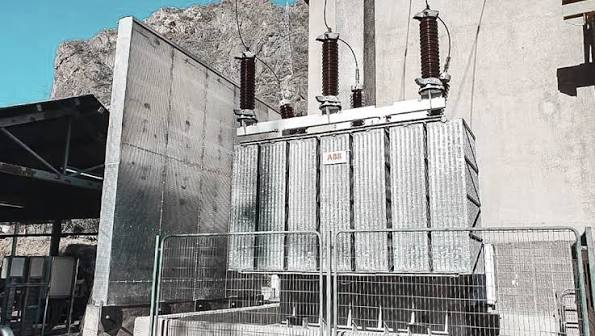
\includegraphics[width=\linewidth, height=4.3cm, keepaspectratio]{pictures/muro_corta_fuegos.jpeg}
      \caption{Muro cortafuego divisorio para transformador.}
    \end{subfigure}%
    \hfill
    \begin{subfigure}[b]{0.40\textwidth}
      \centering
      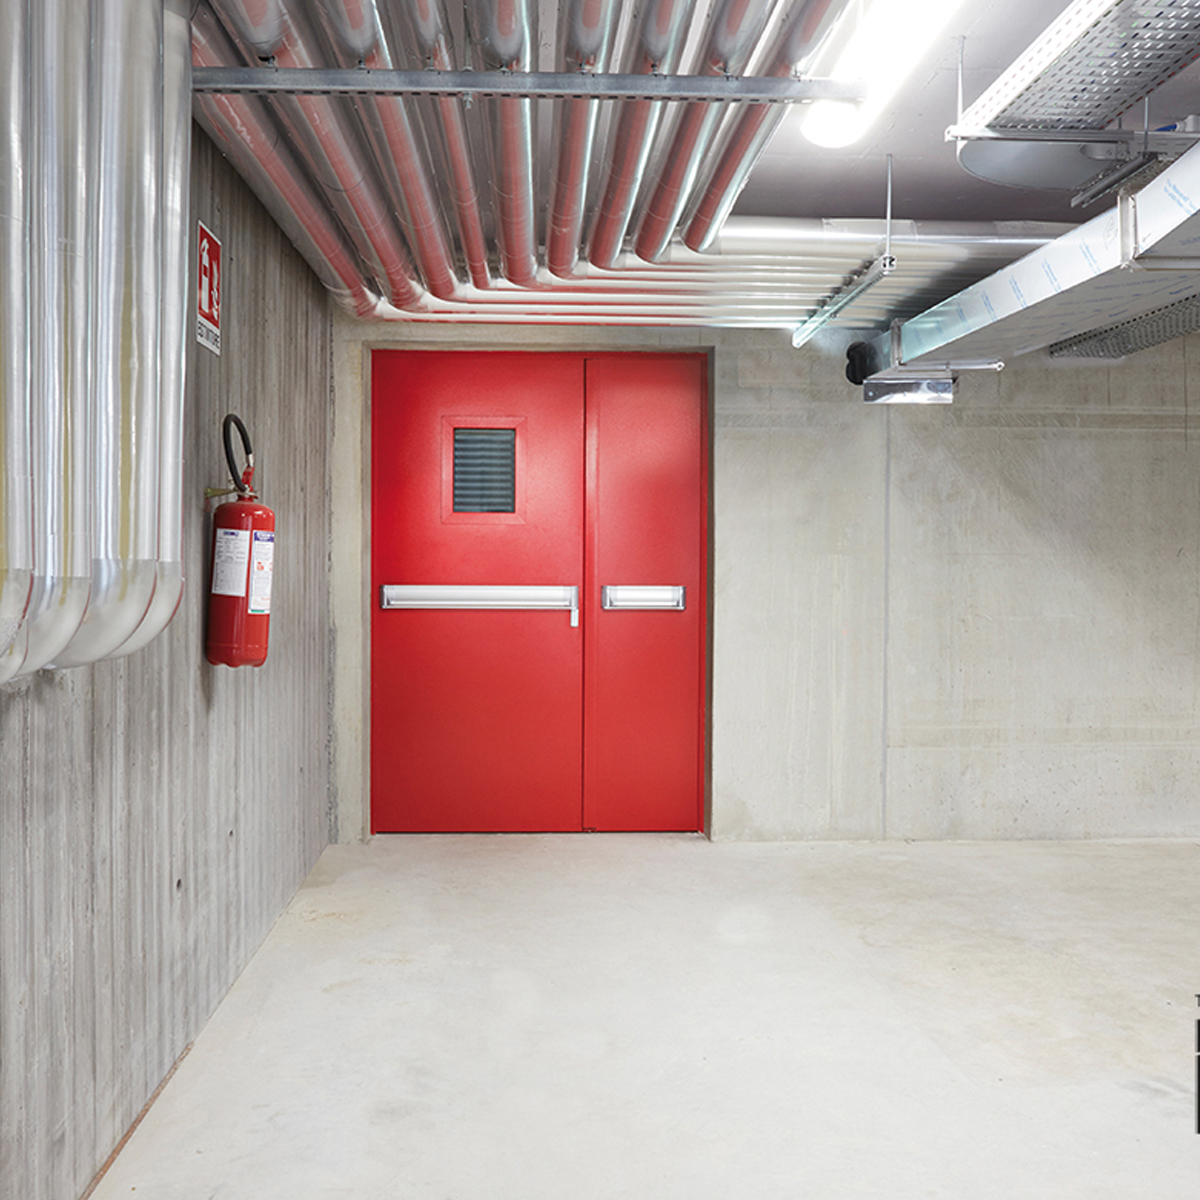
\includegraphics[width=\linewidth, height=4.3cm, keepaspectratio]{pictures/puertas-cortafuegos.jpg}
      \caption{Puertas cortafuego de doble contacto.}
    \end{subfigure}
  \end{figure}
\end{frame}


% --- SLIDE 51 (Pág 53 PDF): ESCALERAS PRESURIZADAS ---
\begin{frame}{Protección Pasiva: Cajas de Escalera Presurizadas para Evacuación}
  \begin{columns}[c]
    \begin{column}{0.50\textwidth}
      \small
      Garantía de rutas de escape libres de humos y gases tóxicos:
      \begin{itemize}
        \scriptsize
        \item En edificios industriales y corporativos, la caja de escaleras se convierte en chimenea de humos si se abre una puerta.
        \item \textbf{Presurización Mecánica Positiva:} Ventiladores de inyección forzada mantienen una sobrepresión continua de $\mathbf{50\,\mathrm{Pa}}$ dentro de la caja de escaleras.
        \item Cuando una puerta de escape se abre hacia la escalera, el gradiente de presión empuja el aire hacia afuera, impidiendo físicamente el ingreso de humos y gases calientes.
      \end{itemize}
    \end{column}

    \begin{column}{0.48\textwidth}
      \centering
      \resizebox{0.85\columnwidth}{!}{%
        \begin{tikzpicture}[scale=0.85]
          \draw[line width=1.5pt, fill=successgreen!10] (0,0) rectangle (2.2,3.5);
          \node[font=\scriptsize\bfseries, align=center] at (1.1,2.8) {Escalera\\$+50\,\mathrm{Pa}$};
          \draw[line width=1.5pt, fill=darkcharcoal!30] (2.2,0) rectangle (4.4,3.5);
          \node[font=\scriptsize\bfseries, align=center] at (3.3,2.8) {Piso con\\Fuego};
          \draw[->, >=stealth, line width=2pt, successgreen!80!black] (1.8,1.2) -- (2.6,1.2);
          \node[above, font=\tiny\bfseries] at (2.2,1.3) {Flujo de Aire Expulsa Humo};
        \end{tikzpicture}
      }
    \end{column}
  \end{columns}
\end{frame}

% --- PROTECCIÓN PASIVA/PREVENTIVA: SEÑALIZACIÓN ---
\begin{frame}{Protección Pasiva/Preventiva: Señalización}
  \begin{columns}[c]
    \begin{column}{0.46\textwidth}
      \small
      Sistema por el cual se facilita la evacuación aún en ausencia total de luz, indicando las salidas, salidas de emergencia, equipos de protección contra incendios, riesgos específicos, etc.
    \end{column}

    \begin{column}{0.52\textwidth}
      \centering
      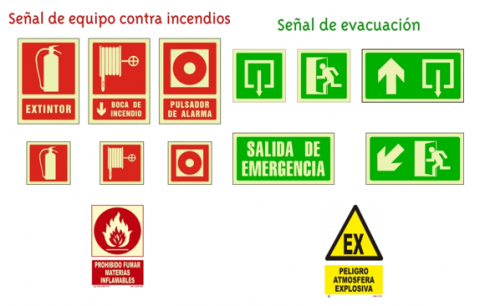
\includegraphics[width=\linewidth, keepaspectratio]{pictures/senalizacion_incendios.png}
    \end{column}
  \end{columns}
\end{frame}

% --- PROTECCIÓN PREVENTIVA: FUENTES DE IGNICIÓN E INSTALACIONES ---
\begin{frame}{Protección Preventiva: Fuentes de Ignición e Instalaciones}
  \begin{itemize}
    \small
    \item \textbf{Instalaciones eléctricas:} Tener en cuenta que la sección de los cables se adapte a la potencia instalada de los artefactos eléctricos a conectar, a fin de evitar cortocircuitos, líneas recargadas, etc.
    \item \textbf{Control de fuentes abiertas:} Apagar correctamente colillas de cigarrillos y fósforos.
    \item \textbf{Equipos térmicos:} Capacitar para el buen manejo de equipos industriales que producen calor y quemadores portátiles.
    \item \textbf{Corte y soldadura:} En trabajos de corte y soldadura mantener los locales ventilados.
    \item \textbf{Electricidad estática:} En operaciones que generen electricidad estática mantener la humedad elevada para evitarla.
  \end{itemize}
\end{frame}

% --- PROTECCIÓN PREVENTIVA: CONTROL DE COMBUSTIBLES Y RESIDUOS ---
\begin{frame}{Protección Preventiva: Control de Combustibles y Residuos}
  \begin{itemize}
    \small
    \item \textbf{Sustancias inflamables:} Almacenar los productos inflamables en lugares ventilados, rotulados y ubicarlos lejos de fuentes de calor.
    \item \textbf{Carga de fuego:} Evitar acumulación de residuos en áreas de trabajos para disminuir la carga de fuego.
    \item \textbf{Materiales y derivados:} Aplicar productos químicos
        ignifugantes, a la madera y sus productos o derivados.
    \item \textbf{Quema en planta:} Evitar la quema de residuos en la planta. Cuando la quema de residuos no pueda evitarse y sea admitida por el Organismo de control, es necesario:
    \begin{itemize}
      \footnotesize
      \item Limitar el lugar.
      \item Tener en cuenta el momento y las condiciones climáticas para hacerlo, y apagarlo cuando cambien las mismas, en especial, respecto al viento.
    \end{itemize}
  \end{itemize}
\end{frame}


% --- SLIDE 44 (Pág 46 PDF): ÉSTERES DIELÉCTRICOS ---
\begin{frame}{Protección Preventiva: Sustitución de Aceite}
  \begin{columns}[c]
    \begin{column}{0.70\textwidth}
      \small
      Riesgo de explosión en transformadores de potencia:
      \begin{itemize}
        \scriptsize
        \item \textbf{Aceite Mineral Convencional:} Hidrocarburo derivado del
            petróleo; punto de inflamación bajo ($140\text{ a }160\,\Celsius$).
              Un arco interno gasifica el aceite provocando fácilmente fuego Clase B.
        \item \textbf{Aceite vegetal o sintético:} Fluidos de clase K basados en
            aceites vegetales refinados o sintéticos:
        \begin{itemize}
          \tiny
          \item \textbf{Punto de fuego $> 300\,\Celsius$ a $> 360\,\Celsius$.}
          \item \textbf{Propiedad autoextinguible:} Si cesa el arco, la llama se extingue sin asistencia.
          \item Reduce drásticamente distancias de seguridad entre transformadores y elimina la necesidad de pesados muros cortafuego masivos.
        \end{itemize}
      \end{itemize}
    \end{column}

    \begin{column}{0.48\textwidth}
      \centering
      \resizebox{0.9\columnwidth}{!}{%
        \begin{tikzpicture}
          \draw[fill=firered!20, draw=firered, line width=1.2pt] (0,1.8) rectangle (4.2,3.2)
                node[midway, font=\scriptsize, align=center] {\textbf{Aceite Mineral}\\Punto Fuego $\approx 160\,\Celsius$\\Explosión violenta Clase B};
          \draw[fill=successgreen!20, draw=successgreen!80!black, line width=1.2pt] (0,0) rectangle (4.2,1.4)
                node[midway, font=\scriptsize, align=center] {\textbf{Aceite
                vegetal o sintético}\\Punto Fuego $> 300\,\Celsius$\\Autoextinguible $\cdot$ Biodegradable};
          \draw[->, >=stealth, line width=2pt, fireorange] (2.1,1.8) -- (2.1,1.4);
        \end{tikzpicture}
      }
    \end{column}
  \end{columns}
\end{frame}

% --- SLIDE 45 (Pág 47 PDF): DISPOSITIVOS AFDD ---
\begin{frame}{Protección Preventiva: Detección de Arco Serie AFDD (IEC 62606)}
  \begin{columns}[c]
    \begin{column}{0.52\textwidth}
      \small
      Límite de las protecciones tradicionales ante arcos serie:
      \begin{itemize}
        \scriptsize
        \item Un conductor fisurado o un borne flojo genera microarcos eléctricos en serie intermitentes.
        \item La corriente de arco en serie está limitada por la propia carga del circuito; \textbf{nunca supera la corriente nominal} ($I_{\mathrm{falla}} < I_n$).
        \item En consecuencia, \textbf{termomagnéticas y disyuntores diferenciales no actúan}.
        \item \textbf{Solución AFDD:} Microcontrolador que analiza la forma de
            onda de la corriente. En caso de detección de anomalía abre el
              circuito rápidamente.
      \end{itemize}
    \end{column}

    \begin{column}{0.45\textwidth}
      \centering
      \resizebox{0.82\columnwidth}{!}{%
        \begin{tikzpicture}[scale=0.8]
          \draw[line width=1pt, ->] (0,0) -- (4.5,0) node[right, font=\tiny] {$t$};
          \draw[line width=1pt, ->] (0,-1.4) -- (0,1.6) node[above, font=\tiny] {$i(t)$};
          % Onda senoidal distorsionada con ruido en el cruce
          \draw[line width=1.2pt, utnblue] (0,0) 
                .. controls (0.5,1.5) .. (1.0,1.2) 
                -- (1.2,0.8) -- (1.3,1.1) -- (1.4,0.7) 
                .. controls (1.8,-0.2) .. (2.2,0)
                .. controls (2.7,-1.5) .. (3.2,-1.2)
                -- (3.4,-0.8) -- (3.5,-1.1) -- (3.6,-0.7)
                .. controls (4.0,0) .. (4.2,0);
          \node[above, font=\tiny\bfseries, firered] at (1.3,1.2) {Ruido RF de Arco};
        \end{tikzpicture}
      }\\[4pt]
      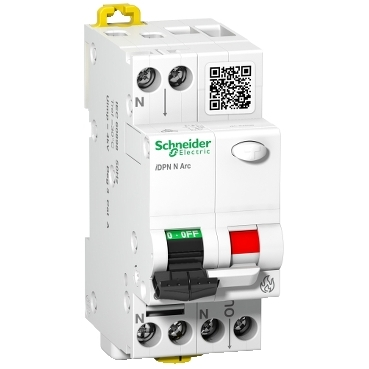
\includegraphics[height=3.0cm, keepaspectratio]{pictures/AFDD.jpg}
    \end{column}
  \end{columns}
\end{frame}

% --- SLIDE 46 (Pág 48 PDF): TERMOGRAFÍA INFRARROJA ---
\begin{frame}{Protección Preventiva: Mantenimiento Predictivo por Termografía}
  \begin{columns}[c]
    \begin{column}{0.50\textwidth}
      \small
      Diagnóstico fallas de origen térmico en tableros:
      \begin{itemize}
        \scriptsize
        \item El aflojamiento mecánico por vibraciones o fatiga térmica genera un aumento de la resistencia en los puntos de contacto.
        \item Por ley de Joule ($P = I^2 R_c$), el borne se calienta progresivamente hasta degradar el aislamiento plástico.
        \item \textbf{Inspección Termográfica Calibrada:} Relevamiento con cámara infrarroja bajo carga nominal del establecimiento.
        \item Gradientes térmicos $\Delta T \ge 10\,\Celsius$ respecto a conductores sanos determinan la intervención preventiva con parada programada.
      \end{itemize}
    \end{column}

    \begin{column}{0.48\textwidth}
      \centering
      \resizebox{0.85\columnwidth}{!}{%
        \begin{tikzpicture}
          \draw[fill=darkcharcoal!20, draw=darkcharcoal, line width=1.2pt] (0,0) rectangle (3.5,2.4);
          \fill[firered] (1.75,1.2) circle (0.5);
          \fill[yellow] (1.75,1.2) circle (0.25);
          \node[font=\tiny\bfseries, white] at (1.75,1.2) {$85\,\Celsius$};
          \node[below, font=\tiny\bfseries] at (1.75,0.4) {Punto Caliente en Borne};
        \end{tikzpicture}
      }
    \end{column}
  \end{columns}
\end{frame}

% --- SLIDE 52: BRIGADAS EPI Y ESI ---
\begin{frame}{Organización Humana de Respuesta: E.P.I. y E.S.I.}
  \small
  Estructura escalonada para la gestión humana de emergencias (doctrina de cátedra y SRT):

  \vspace{0.4cm}
  \centering
  \begin{tikzpicture}[
    line cap=round, line join=round,
    boxcomite/.style={draw=darkcharcoal, fill=cardbg, line width=1.3pt, rounded corners=5pt, text width=7.4cm, align=center, inner sep=6pt},
    boxepi/.style={draw=firered, fill=firered!12, line width=1.3pt, rounded corners=5pt, text width=5.7cm, align=center, inner sep=6pt},
    boxesi/.style={draw=utnblue, fill=utnblue!12, line width=1.3pt, rounded corners=5pt, text width=5.7cm, align=center, inner sep=6pt}
  ]
    % Comité (arriba centro)
    \node[boxcomite] (Comite) at (0, 1.8) {
      {\small\textbf{\textcolor{darkcharcoal}{Comité de Emergencia y Jefe de Emergencia}}}\\[3pt]
      {\scriptsize Conducción estratégica $\;\cdot\;$ Orden de evacuación $\;\cdot\;$ Punto de encuentro}
    };

    % EPI (abajo izquierda)
    \node[boxepi] (EPI) at (-3.65, -0.8) {
      {\small\textbf{\textcolor{firered}{Equipo de Primera Intervención (E.P.I.)}}}\\[3pt]
      {\scriptsize Fuerza de choque en taller $\;\cdot\;$ Advertencia\\[2pt] Extintores en $<30\,\mathrm{s}$}
    };

    % ESI (abajo derecha)
    \node[boxesi] (ESI) at (3.65, -0.8) {
      {\small\textbf{\textcolor{utnblue}{Equipo de Segunda Intervención (E.S.I.)}}}\\[3pt]
      {\scriptsize Brigada de planta $\;\cdot\;$ Mangueras $45/63.5\mm$\\[2pt] ERA $\;\cdot\;$ Bomberos}
    };

    % Conexiones jerárquicas desde Comité
    \coordinate (fork) at (0, 0.5);
    \draw[line width=1.3pt, darkcharcoal] (Comite.south) -- (fork);
    \draw[->, >=stealth, line width=1.3pt, darkcharcoal] (fork) -| (EPI.north);
    \draw[->, >=stealth, line width=1.3pt, darkcharcoal] (fork) -| (ESI.north);

    % Coordinación operativa entre EPI y ESI
    \draw[<->, >=stealth, line width=1.3pt, dashed, darkcharcoal!80] (EPI.east) -- (ESI.west);

  \end{tikzpicture}
\end{frame}

% --- SLIDE 43: JERARQUÍA DE CONTROL DE RIESGOS ---
\begin{frame}{La Jerarquía de Control de Riesgos (ISO 45001 / IRAM 3800)}
  \begin{columns}[c]
    \begin{column}{0.48\textwidth}
      \small
        Jerarquía de medidas según efectividad (de mayor a menor prioridad):
      \begin{enumerate}
        \scriptsize
        \item \textbf{Eliminación:} Suprimir físicamente el peligro en el diseño.
        \item \textbf{Sustitución:} Reemplazar reactivos y fluidos combustibles por alternativas no inflamables.
        \item \textbf{Controles de Ingeniería:} Salvaguardas tecnológicas automáticas, AFDD, termografía, ventilación forzada.
        \item \textbf{Controles Administrativos:} Protocolos de trabajo seguro, permisos PTC y metodología 5S.
        \item \textbf{EPP:} Atenuación del impacto residual sobre el trabajador.
      \end{enumerate}
    \end{column}

    \begin{column}{0.50\textwidth}
      \centering
      \resizebox{0.95\columnwidth}{!}{%
        \begin{tikzpicture}[yscale=0.7]
          \draw[fill=firered!80, line width=1pt] (0,4) rectangle (5.4,4.7) node[midway, text=white, font=\scriptsize\bfseries] {1. Eliminación};
          \draw[fill=fireorange!80, line width=1pt] (0.3,3) rectangle (5.1,3.7) node[midway, text=white, font=\scriptsize\bfseries] {2. Sustitución};
          \draw[fill=amberyellow!85!black, line width=1pt] (0.6,2) rectangle (4.8,2.7) node[midway, text=white, font=\scriptsize\bfseries] {3. Controles de Ingeniería};
          \draw[fill=utncyan, line width=1pt] (0.9,1) rectangle (4.5,1.7) node[midway, text=white, font=\scriptsize\bfseries] {4. Controles Administrativos};
          \draw[fill=utnblue, line width=1pt] (1.6,0) rectangle (3.8,0.7) node[midway, text=white, font=\scriptsize\bfseries] {5. EPP};
        \end{tikzpicture}
      }
    \end{column}
  \end{columns}
\end{frame}

% --- SLIDE 53: CASO IRON MOUNTAIN ---
\begin{frame}{Análisis Forense: Depósito Iron Mountain (Barracas, 2014)}
  \begin{columns}[c]
    \begin{column}{0.50\textwidth}
      \small
      Lecciones del colapso estructural de Barracas:
      \begin{itemize}
        \scriptsize
        \item \textbf{Carga de fuego extrema ($Q_f \gg 150\,\kg/\m^2$):} Racks metálicos autoportantes de más de $10\,\m$ densamente cargados de papel.
        \item \textbf{Efecto tiro de chimenea vertical:} Aceleración violenta de las llamas hacia el techo.
        \item \textbf{Falla activa total:} Válvulas de rociadores cerradas sin presurización; bombas principales apagadas.
        \item \textbf{Ausencia de protección pasiva en el acero:} Al superar los $900\,\Celsius$, el acero sufrió fluencia térmica, pandeó y empujó el muro este hacia la calle Jovellanos, provocando el fallecimiento de 10 rescatistas.
      \end{itemize}
    \end{column}

    \begin{column}{0.48\textwidth}
      \centering
      \resizebox{0.85\columnwidth}{!}{%
        \begin{tikzpicture}
          \draw[line width=1.5pt, fill=firered!10] (0,0) rectangle (3.5,3.0);
          \draw[line width=2pt, dashed, firered] (0,0) -- (-0.8,2.8) node[above, font=\tiny\bfseries, firered] {Colapso hacia la calle};
          \node[font=\tiny\bfseries, align=center] at (1.75,1.5) {Fluencia térmica a $>900\,\Celsius$\\Pandeo de cabriadas\\Empuje sobre muro exterior};
        \end{tikzpicture}
      }
    \end{column}
  \end{columns}
\end{frame}

% --- SLIDE 54: CASO EDESUR CABALLITO ---
\begin{frame}{Análisis Forense: Subestación Edesur Caballito (2024)}
  \begin{columns}[c]
    \begin{column}{0.50\textwidth}
      \small
      Falla durante mantenimiento electromecánico:
      \begin{itemize}
        \scriptsize
        \item Intervención sobre transformador de $132/13.2\,\mathrm{kV}$ con máquina de filtrado de aceite caliente.
        \item Rotura de manguera flexible bajo presión: pulverización de aceite mineral sobre bornes calientes/energizados.
        \item \textbf{Fuego mixto Clase B + Clase C:} Propagación inmediata por túneles y bandejas de cables aislados con PVC convencional.
        \item Columnas densas de humo negro y $HCl$ bloquearon la visibilidad y demoraron el ataque.
        \item \textbf{Lección de diseño:} Obligatoriedad de ésteres dieléctricos autoextinguibles y conductores LS0H en subestaciones urbanas.
      \end{itemize}
    \end{column}

    \begin{column}{0.48\textwidth}
      \centering
      \resizebox{0.85\columnwidth}{!}{%
        \begin{tikzpicture}
          \draw[fill=darkcharcoal!20, line width=1.2pt] (0,0) rectangle (3.2,2.2) node[midway, font=\tiny\bfseries] {Transformador de Potencia};
          \draw[->, >=stealth, line width=2pt, firered] (3.2,1.1) -- (4.2,1.1) node[right, font=\tiny\bfseries, firered] {Fuga de Aceite};
          \node[below, font=\tiny\bfseries] at (1.6,-0.2) {Propagación por cables de PVC};
        \end{tikzpicture}
      }
    \end{column}
  \end{columns}
\end{frame}

% --- SLIDE 55: MATRIZ RESUMEN Y CONCLUSIONES ---
\begin{frame}{Matriz Síntesis de Soluciones y Conclusiones Finales}
  \small
  La prevención y protección eficaz conforma un sistema integral de barreras múltiples:

  \vspace{0.2cm}
  \begin{table}[h]
    \centering
    \scriptsize
    \begin{tabular}{p{2.8cm} p{2.2cm} p{3.4cm} p{3.2cm}}
      \toprule
      \textbf{Medida de Solución} & \textbf{Nivel / Tipo} & \textbf{Mecanismo Técnico} & \textbf{Impacto Operativo} \\
      \midrule
      \textbf{Ésteres Dieléctricos} & Sustitución / Prev. & Punto de fuego $>300\,\Celsius$, autoextinguible & Elimina explosión Clase B en transformadores. \\
      \addlinespace
      \textbf{Cables LS0H} & Sustitución / Prev. & Poliolefinas sin halógenos; vapor no tóxico & Mantiene visibilidad y evita corrosión de silicio. \\
      \addlinespace
      \textbf{Dispositivos AFDD} & Ingeniería / Prev. & Detección de firma de RF de arco serie & Evita arcos que burlan a termomagnéticas. \\
      \addlinespace
      \textbf{Sectorización $F$} & Ingeniería / Pasiva & Muros certificados y sellos intumescentes & Confinamiento físico del fuego y gases calientes. \\
      \addlinespace
      \textbf{Brigadas E.P.I. / E.S.I.} & Humana / Activa & Advertencia precoz y ataque con hidrantes & Ataque en $<30\,\mathrm{s}$ y enlace con bomberos. \\
      \bottomrule
    \end{tabular}
  \end{table}
\end{frame}
